\documentclass[a4paper]{amsart}

\usepackage[]{graphicx}

\setlength{\parindent}{0.0in}
\setlength{\parskip}{0.1in}

\newcommand{\laplace}[1]{\mathcal{L}\{#1\}}
\newcommand{\Hv}{\textrm{H}}

\begin{document}
\title{6G5Z3011 Multi-variable calculus and analytical methods}
\author{Tutorial Sheet 01}
\maketitle

\begin{enumerate}
\item
Find the first derivatives of the following functions
\begin{enumerate}
\item
$f(x,y)=3x^2 \text{ln}(y)$
\item
$g(x,y)=4y \sin (x^2 + 2y)$
\item
$h(x,y,z) = 7x^2 y + \frac{1}{z} + xyz + 2$   
\end{enumerate}
\item
Given that $f(x,y)= \text{ln} (x^2 + y^2)$, show that 
\begin{enumerate}
\item
$$\frac{\partial^2 f}{\partial x \partial y} = \frac{\partial^2 f}{\partial y \partial x}$$
\item
$$\frac{\partial^2 f}{\partial x^2} + \frac{\partial^2 f}{\partial y^2} =0$$
\end{enumerate}
\item
Consider the function $f$ defined by 
$$ f(x,y)=x^2 y^3 .$$
Show using the limit definition of the partial derivative that $\frac{\partial f}{\partial x} = 2xy^3$ and $\frac{\partial f}{\partial y}=3x^2 y^ 2$.
\item
Consider a hill whose height above sea level at a point $x$km east and $y$km north of its peak is given by the value $z(x,y)$ of the function $z$ defined by 
$$z(x,y) = 1000 e^{-u} + 110 \text{ metres},$$
where $u=x^2 + y^2$. Plot the 400, 600, ... , 1000 metre contours of this hill on a map.



Find the coordinates of the point $P$, due noth west of the peak, which is exactly 400 metres above sea level, and mark it on your plot. What is the slope of the hill at this point $P$, in a (i) northerly direction, and in an (ii) easterly direction.

\item
Demonstrate that the dunction $\phi$, defined by
$$\phi(x,y) = e^x \sin(y)$$
is a solution of Laplace's differential equation
$$\frac{\partial^2 \phi}{\partial x^2} + \frac{\partial^2 \phi}{\partial y^2} = 0.$$
\item
Demonstrate that the function $\psi$, defined by
$$\psi(x,y,t) = e^{-t} (\sin(x) + \cos(y)),$$
is a solution of the partial differentiatial equation
$$\frac{\partial^2 \psi}{\partial x^2}+\frac{\partial^2 \psi}{\partial y^2}
= \frac{\partial \psi}{\partial t}.$$
\item
Find all the locations $(x,y)$ where the two partial derivatives $\frac{\partial f}{\partial x}$ and $\frac{\partial f}{\partial y}$ are simultaneously zero, where $f$ is the function defined by
$$f(x,y) = \cos(x^2+y^2).$$
\item
Use the technique of implicit partial differentiation to find expressions for $\frac{\partial z}{\partial x}$ and $\frac{\partial z}{\partial y}$ where $x,y,z$ are related by the condition
$$xy + yz + zx = 1.$$
\item
Consider the 1-dimensional heat equation
$$\frac{\partial u}{\partial t} - \frac{\partial^2 u}{\partial x^2} = 0$$
which describes the distribution of heat in a region at time $t$. Show that the function $u$ defined by $$u(x,t) = e^{-\beta t} \sin (\alpha x)$$
is a solution of the heat equation when a certain relationship holds between the parameters $\alpha$ and $\beta$.
\item
Consider a general triangle with angles $A,B,C$ whose opposite sides have lengths $a,b,c$ respectively.

Find an expression that gives the rate of change of angle $A$ as side length $a$ is varied, but $b$ and $c$ are kept fixed. To do this make use of implicit differentiation and the cosine formula
$$a^2 = b^2 + c^2 - 2bc \cos(A).$$

\end{enumerate}
\vfill
\begin{center}
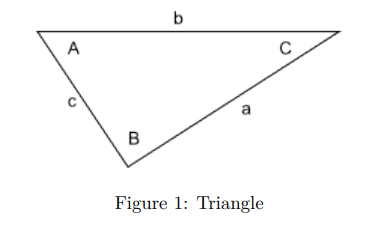
\includegraphics[scale=0.5]{triangle.png}
\end{center}
\vfill





\end{document}